
\section{Ladungen im elektromagnetischen Feld
\label{relativ:section:em_feld}}
\kopfrechts{Ladungen im elektromagnetischen Feld}

In diesem Abschnitt soll die Berechnung des Verhaltens eines Elementarteilchens
unter der Einwirkung eines elektromagnetischen Feldes erläutert werden.


\subsection{Bewegungsgleichung
\label{relativ:section:bewegungsgleichung}}

Bei der Berechnung der Bahn eines Elementarteilchens
in einem elektromagnetischen Feld geht man von
der vereinfachenden, aber angemessenen Annahme aus,
dass die Rückwirkung des Teilchens auf das Feld vernachlässigt werden kann\footnote{
Konkret muss für diese Annahme beispielsweise
für die magnetische Feldstärke
\(H \ll \frac{m^2c^4}{e^3}\) erfüllt sein.
Die rechte Seite ergibt dabei für ein Elektron
eine magnetische Feldstärke von
\(\frac{m_e^2c^4}{e^3} \approx
\frac{(\qty{9e-31}{\kilogram})^2 (\qty{3e8}{\metre\per\second})^4}{(\qty{1.6e-19}{\ampere\second})^3}
\approx \qty[per-mode=fraction]{1.6e30}{\ampere\per\metre}\),
was im Vakuum einer magnetischen Flussdichte von
\(\mu_0 \cdot \qty[per-mode=fraction]{1.6e30}{\ampere\per\metre} \approx
\qty[per-mode=fraction]{1.25e-6}{\tesla\metre\per\ampere} \cdot
\qty[per-mode=fraction]{1.6e30}{\ampere\per\metre} =
\qty{2e24}{\tesla}\)
entspricht, einem Wert weitaus grösser als alle bekannten physikalischen Phänomene.}.

Die Bewegungsgleichung ergibt sich aus der Variation des Wirkungsintegrals
mit der Euler-Lagrange-Differentialgleichung
\begin{equation}
    \frac{d}{dt} \frac{\partial L}{\partial \bm{v}} - \frac{\partial L}{\partial \bm{r}} = 0,
    \label{relativ:eqn:euler-lagrange-em-feld}
\end{equation}
wobei \(L\) in \eqref{relativ:eqn:lagrange-em-feld} gegeben ist.
Die Ableitung nach dem Geschwindigkeitsvektor \(\bm{v}\) ergibt
\begin{equation}
    \frac{\partial L}{\partial \bm{v}} =
    mc^2 \frac{-\frac{2}{c^2}\bm{v}}{-2\sqrt{1-\frac{v^2}{c^2}}}
    + \frac{e}{c} \bm{A} - 0
    = \frac{m \bm{v}}{\sqrt{1-\frac{v^2}{c^2}}} + \frac{e}{c} \bm{A}.
    \label{relativ:eqn:part-diff-v}
\end{equation}
Dies wird auch als verallgemeinerter Teilchenimpuls \(\bm{P}\) bezeichnet,
wovon der linke Term der gewöhnliche (relativistische) Impuls \(\bm{p}\)
des Teilchens ist.
Vergleicht man diesen mit dem Impuls der klassischen Mechanik, \(m\bm{v}\),
so unterscheidet er sich um den wiederkehrenden Faktor
\(\gamma=\frac{1}{\sqrt{1-v^2/c^2}}\), den sogenannten \emph{Lorentz-Faktor}.
\index{Lorentz-Faktor}%
Der Gesamtausdruck \(\frac{m}{\sqrt{1-v^2/c^2}}\) wird auch als
relativistische Masse \(m^*\) bezeichnet. Somit kann beispielsweise der
Impuls analog zur gewöhnlichen Mechanik als
\(\bm{p}=m^*\bm{v}\) geschrieben werden\footnote{
    In diesem Zusammenhang wird die Ruhemasse eines Objekts, d.h.
    die Masse, die ein Körper hat, wenn er in Ruhe ist,
    als \(m_0\) bezeichnet.
    Wir werden hier bei der Bezeichnung \(m\) bleiben.
}.

Die partielle Ableitung von \(L\) nach \(\bm{r}\) ergibt dann
\begin{equation}
    \frac{\partial L}{\partial \bm{r}} = \nabla L
    = 0 + \frac{e}{c} \operatorname{grad} \bm{Av} - e \operatorname{grad} \varphi.
    \label{relativ:eqn:part-diff-r}
\end{equation}
Wir können nun \eqref{relativ:eqn:part-diff-v} und \eqref{relativ:eqn:part-diff-r}
in \eqref{relativ:eqn:euler-lagrange-em-feld} einsetzen und erhalten
\begin{equation}
    \frac{d}{dt} \biggl(\bm{p} + \frac{e}{c} \bm{A}\biggr)
    - \frac{e}{c} \operatorname{grad} \bm{Av} + e \operatorname{grad} \varphi = 0.
    \label{relativ:eqn:euler-lagrange-em-eingesetzt}
\end{equation}
Diese Differentialgleichung kann mittels Formeln der Vektoranalysis
umgeformt werden, um schliesslich
\begin{equation}
    \frac{d\bm{p}}{dt} = -\frac{e}{c} \frac{\partial\bm{A}}{\partial t}
    - e \operatorname{grad} \varphi +
    \frac{e}{c} \bm{v} \times \operatorname{rot} \bm{A}
    \label{relativ:eqn:euler-lagrange-em-umgeformt}
\end{equation}
zu erhalten.

\subsection{Beispiel mit einem statischen elektrischen Feld
\label{relativ:section:teilchen-konst-e-feld}}

Gehen wir von der einfachen Situation aus,
in der sich ein Elektron durch ein statisches
elektrisches Feld bewegt und \(\bm{A}\)
somit dem Nullvektor entspricht.
Der Geschwindigkeitsvektor des Elektrons zu Beginn sei
\(\bm{v}_0 = \bm{v}(t=0) =(\beta_0 c, 0, 0)^T\), wobei
\(\beta_0 \in (0, 1)\).

\subsubsection{Euler-Lagrange-Differentialgleichung}
Die Differentialgleichung aus \eqref{relativ:eqn:euler-lagrange-em-umgeformt} reduziert sich zu
\begin{equation}
    \frac{d\bm{p}}{dt} =
    - e \operatorname{grad} \varphi.
    \label{relativ:eqn:euler-lagrange-bsp-1}
\end{equation}
In einem nächsten Schritt wird für \(\bm{p}\)
wieder der Ausdruck aus \eqref{relativ:eqn:part-diff-v} eingesetzt,
womit
\begin{equation}
    \frac{d\bm{p}}{dt} =
    \frac{d}{dt} \Biggl(\frac{m_e}{\sqrt{1-\frac{v^2}{c^2}}} \bm{v}\Biggr) =
    - e \operatorname{grad} \varphi,
    \label{relativ:eqn:euler-lagrange-bsp-eingesetzt}
\end{equation}
mit der Elektronenmasse \(m_e\) und der Elementarladung \(e\).
\index{Elektronenmasse}%
\index{Elementarladung}%
\index{e@$e$, Elementarladung}%
Die Ableitung des Impulses entspricht somit lediglich
dem Gradienten des elektrischen Potentials, oder dem elektrischen Feld.
Der wesentliche Unterschied zur klassischen Mechanik ist hierbei
der bekannte Lorentz-Faktor \(\gamma\).

Die zeitliche Ableitung des Ausdrucks in der Klammer ist nicht ganz trivial,
da \(v^2=\sqrt{\bm{v}\cdot\bm{v}}\)
und somit natürlich auch von \(t\) abhängt.
Zur Vereinfachung der folgenden Rechnung führen wir an dieser Stelle
die Geschwindigkeit in Einheiten der Vakuumlichtgeschwindigkeit ein:
\begin{equation*}
    \bm{\beta} := \frac{\bm{v}}{c} \quad \text{und} \quad
    \beta = \sqrt{\bm{\beta}\cdot\bm{\beta}} = \frac{v}{c}.
\end{equation*}
Mittels Quotientenregel ergibt sich dann
\begin{align*}
    \frac{d\bm{p}}{dt}
    &= \frac{d}{dt} \Biggl(\frac{m_e \bm{v}}{\sqrt{1-\frac{v^2}{c^2}}}\Biggr)
    = \frac{d}{dt} \Biggl(\frac{m_e c \bm{\beta}}{\sqrt{1-\beta^2}}\Biggr)
    = \frac{m_ec\frac{d\bm{\beta}}{dt}\sqrt{1-\beta^2}
    -m_ec\bm{\beta}\cdot\frac{-\cancel{2}\bm{\beta}}{\cancel{2}\sqrt{1-\beta^2}}
    \frac{d\bm{\beta}}{dt}}{1-\beta^2}\\
    &= m_ec\frac{d\bm{\beta}}{dt}\frac{\bigl(1-\beta^2\bigr)^\frac{1}{2}
    +\bm{\beta}\cdot\bm{\beta} \ \bigl(1-\beta^2\bigr)^{-\frac{1}{2}}}
    {\bigl(1-\beta^2\bigr)^1}
    = m_ec\frac{d\bm{\beta}}{dt}\frac{\bigl(1-\beta^2\bigr)^1
    +\beta^2}{\bigl(1-\beta^2\bigr)^\frac{3}{2}}
    = \frac{m_ec}{\bigl(1-\beta^2\bigr)^\frac{3}{2}}\frac{d\bm{\beta}}{dt}.
\end{align*}

Nehmen wir nun beispielsweise an,
dass das elektrische Feld lediglich eine \(x\)-Kom"-po"-nen"-te hat,
sprich \( \operatorname{grad} \varphi = (-E_x, 0, 0)^T \),
so ergibt sich für die Ableitung des Geschwindigkeitsvektors
\begin{equation}
    \frac{d}{dt}
    \begin{pmatrix}
        v_x \\
        v_y \\
        v_z
    \end{pmatrix} =
    \frac{d}{dt} c
    \begin{pmatrix}
        \beta_x \\
        \beta_y \\
        \beta_z
    \end{pmatrix}
    =
    - \frac{e \bigl(1-\beta^2\bigr)^\frac{3}{2}}{m_e}
    \begin{pmatrix}
        -E_x \\
        0 \\
        0
    \end{pmatrix}.
    \label{relativ:eqn:bsp-abl-v-vec}
\end{equation}
Hierbei ist klar, dass sich die Geschwindigkeitskomponenten
in \(y\)- und \(z\)-Richtung nicht ändern können.
Zusammen mit der Anfangsgeschwindigkeit \(\bm{v}_0\)
ergibt sich somit die nichtlineare Differentialgleichung erster Ordnung
\begin{equation}
    \frac{d\beta_x}{dt} = \frac{e E_x}{c m_e} \bigl(1-\beta_x^2\bigr)^\frac{3}{2}
    := \eta \, \bigl(1-\beta_x^2\bigr)^\frac{3}{2}
\end{equation}
für die Geschwindigkeit \(\beta_x\) in \(x\)-Richtung,
wobei der Übersicht halber die Konstante
\(\eta=\frac{e E_x}{c m_e}\) eingeführt wurde.
Diese Differentialgleichung kann mittels Separierung gelöst werden.
Wir separieren nach den Variablen \(\beta_x\) und \(t\)
und integrieren auf beiden Seiten:
\begin{align*}
    \int\frac{d\beta_x}{\bigl(1-\beta_x^2\bigr)^\frac{3}{2}}
    &= \int\eta dt \\
    \Rightarrow\qquad\frac{\beta_x}{\sqrt{1-\beta_x^2}}
    &= \eta t + K_1,
\end{align*}
mit der Integrationskonstanten \(K_1\).
Diese Gleichung kann nun nach \(\beta_x\) aufgelöst werden:
\begin{equation*}
\begin{aligned}
    &&
    \frac{\beta_x^2}{1-\beta_x^2}
    &= \bigl(\eta t + K_1\bigr)^2
\\
&\Leftrightarrow&
\beta_x^2 &= \bigl(\eta t + K_1\bigr)^2
\bigl(1-\beta_x^2\bigr)
\\
&\Leftrightarrow&\qquad
\beta_x^2 \bigl(1 + \bigl(\eta t + K_1\bigr)^2\bigr)
&= \bigl(\eta t + K_1\bigr)^2
\\
    &\Leftrightarrow&
    \beta_x^2 &= \frac{\bigl(\eta t + K_1\bigr)^2}
    {1 + \bigl(\eta t + K_1\bigr)^2}
\\
    &\Leftrightarrow&
    \beta_x(t) &= \frac{\eta t + K_1}
    {\sqrt{1+\bigl(\eta t+K_1\bigr)^2}}.
\end{aligned}
\end{equation*}

\subsubsection{Anfangsbedingungen}
Mit der Anfangsbedingung \(\beta_x(t=0)=\beta_0\) erhält man
\begin{align*}
\beta_x(0)
&=
\beta_0 = \frac{K_1}{\sqrt{1+K_1^2}}
&
&\Leftrightarrow
&
K_1^2
&=
\beta_0^2 \bigl(1+K_1^2\bigr)
&
&&&
\\
&
&
&\Leftrightarrow
&
K_1^2 (1-\beta_0^2 )
&=
\beta_0^2 
&
&\Leftrightarrow
&
K_1
&=
\frac{\beta_0}{\sqrt{1-\beta_0^2 }}
\end{align*}
und somit eine vollständige Gleichung für die Geschwindigkeit des Elektrons.
In Abbildung~\ref{relativ:fig:elektron-em-feld} ist die Gleichung für einige
Werte von \(\beta_0\) und \(E_x\) dargestellt.
\begin{figure}
    \centering
    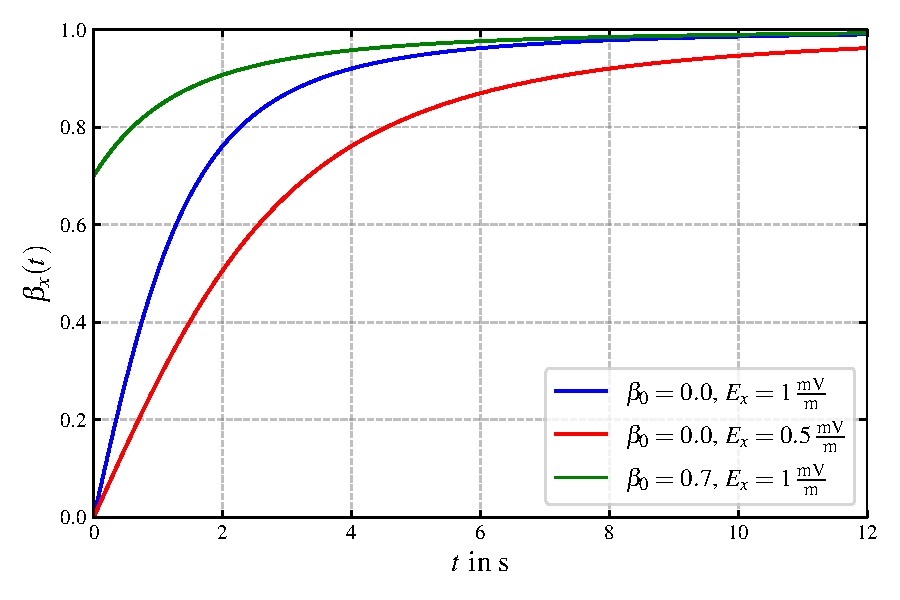
\includegraphics[width=0.8\linewidth]{papers/relativ/images/elektron_e-feld.pdf}
    \caption{Geschwindigkeit in Einheiten der Vakuumlichtgeschwindigkeit
    eines Elektrons in einem statischen elektrischen Feld in Abhängigkeit der Zeit \(t\),
    für verschiedene Feldstärken \(E_x\) und Startgeschwindigkeiten \(\beta_0 c\).
    \label{relativ:fig:elektron-em-feld}}
\end{figure}

\subsubsection{Diskussion}
An den Ergebnissen der Rechnung sieht man, dass das Elektron (und tatsächlich auch kein anderes
massebehaftetes Teilchen) nicht über die Lichtgeschwindigkeit \(c\) hinaus beschleunigt werden kann.
Je näher das Elektron der Lichtgeschwindigkeit kommt, desto mehr sieht es so aus,
als würde es immer schwerer werden anstatt weiter zu beschleunigen.
Dies ist natürlich dem Lorentz-Faktor in Gleichung~\eqref{relativ:eqn:euler-lagrange-bsp-eingesetzt}
zu verdanken.

Diese Eigenschaft wird in Teilchenbeschleunigern wie dem LHC\footnote{
\index{LHC}%
\index{Large Hadron Collider}%
Der \emph{Large Hadron Collider} (LHC) ist der leistungsstärkste
Teilchenbeschleuniger der Welt und befindet sich am
\index{Teilchenbeschleuniger}%
Kernforschungszentrum CERN bei Genf.
\index{CERN}%
}
dazu verwendet, um eine hohe Menge Energie in Elementarteilchen zu bringen.
Da die Teilchen dabei irgendwann nicht mehr schneller werden
(sondern nur noch ``schwerer''),
können sie stets mit Strahlung derselben Frequenz angeregt werden, und
diese muss nicht an die Geschwindigkeit angepasst werden.
